\section{Motivation and Background}

%When people analyze large size of data, parallel programme is widely used in order to reduce computation time, especially when using supercomputer.
%However, it is usually difficult for a non-computer-scientist to write a parallel program, or re-write some existing applications into parallel version.
%Many serial applications are submitted to Supercomputer and occupy computing nodes for a long time, causing other applications which offer large number of nodes to wait for nodes, and leading a low utilization of computing resource.
%Consider following situation, there are 50 nodes available when a user submits a serial program using 1 node for 4 hours, after an hour a user try to run a program using 50 nodes, then he can't start his program until the first user finished his job.
%Such situation happens frequently when thousands and hundreds of users using one system at the same time and leading a low utilization of computing resource.
%One solution is running several virtual machines on a single physical machine for increasing utilization, which is used in TSUBAME Supercomputer, but sometime it still can't meet the request.
%For request not always reaches peak, it is not wise to increase nodes just for a temporary request peak.
%However even using virtual machines computing nodes still can't meet the request of users, for example, power problem will be critical in summer and nearly half of computing nodes have be shut down to reduce electricity consumption in the case of TSUBAME Supercomputer.
%Facing these problems, one solution will be federate supercomputer with public cloud.
%By using public cloud computing nodes just in request peak or when facing with power problem, people can save cost for buying new machines.
%Of cause, there will be many challenges when Supercomputer federates with public cloud, such as security problems, using public cloud may cause research data opened to public, also connecting with Internet put Supercomputer under threats of hacker's attack.

%Data shown in this section is taken from AMAZON EC2 m3.medium nodes, which have 3.75GiB memory and Moderate Network Performance and TSUBAME 2.5 V queue, which uses VM.
\begin{figure}[tb]
	\centering
	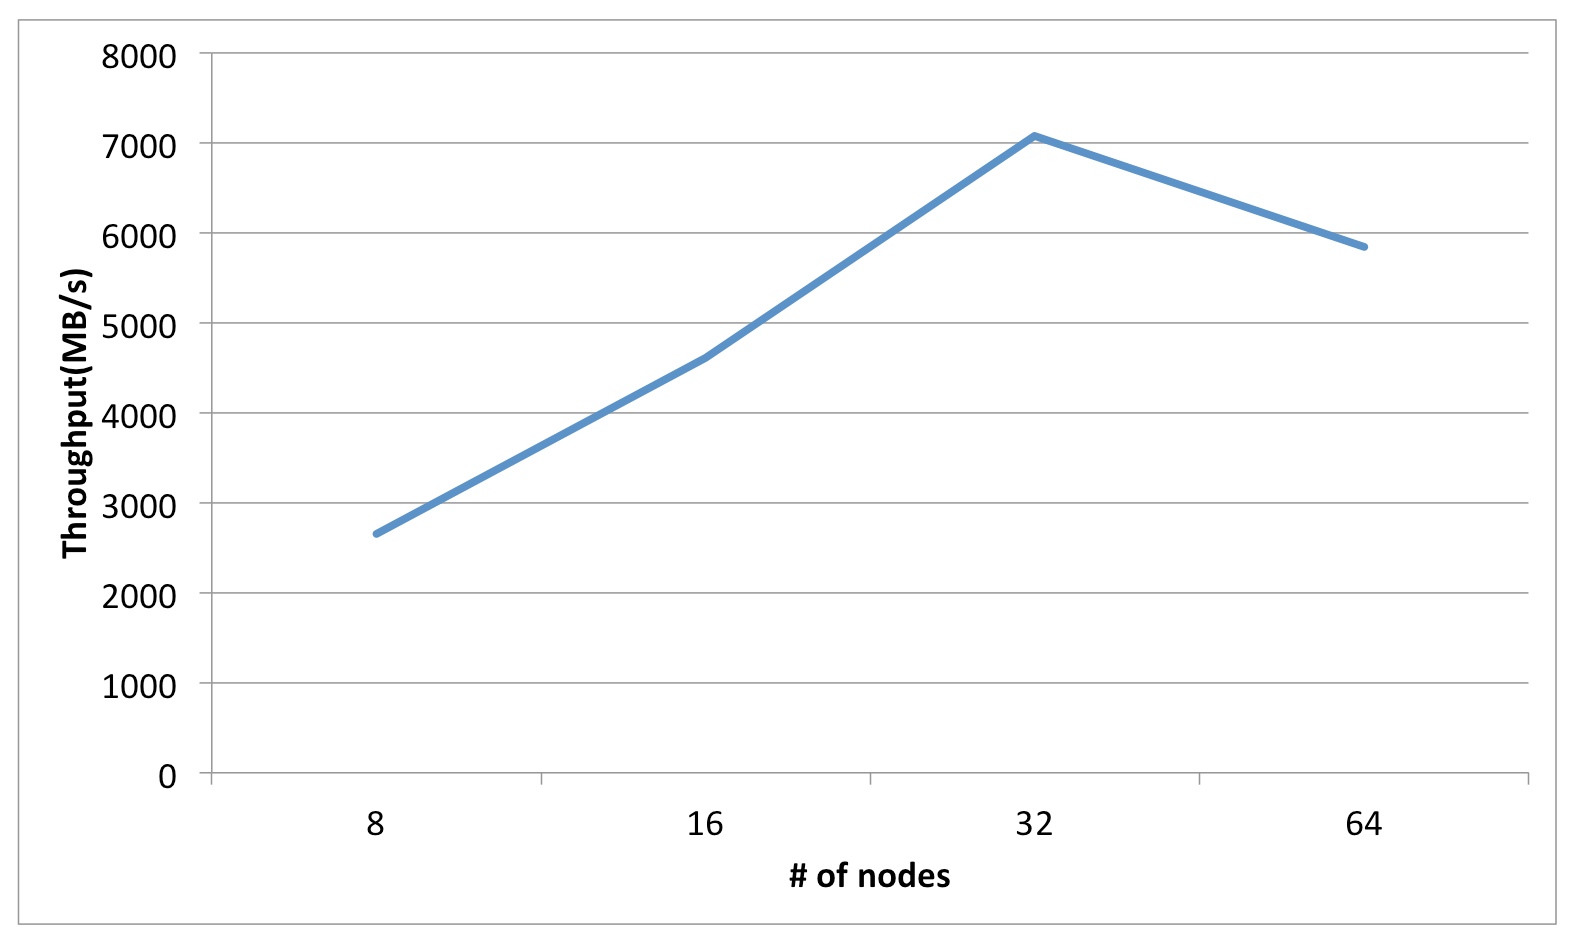
\includegraphics[width=6cm]{../img/throughput_tsubame}
	\caption{I/O Throughput to Lustre inside TSUBAME direct mount}
	\label{throughput TSUBAME}
\end{figure}

\begin{figure}[tb]
	\centering
	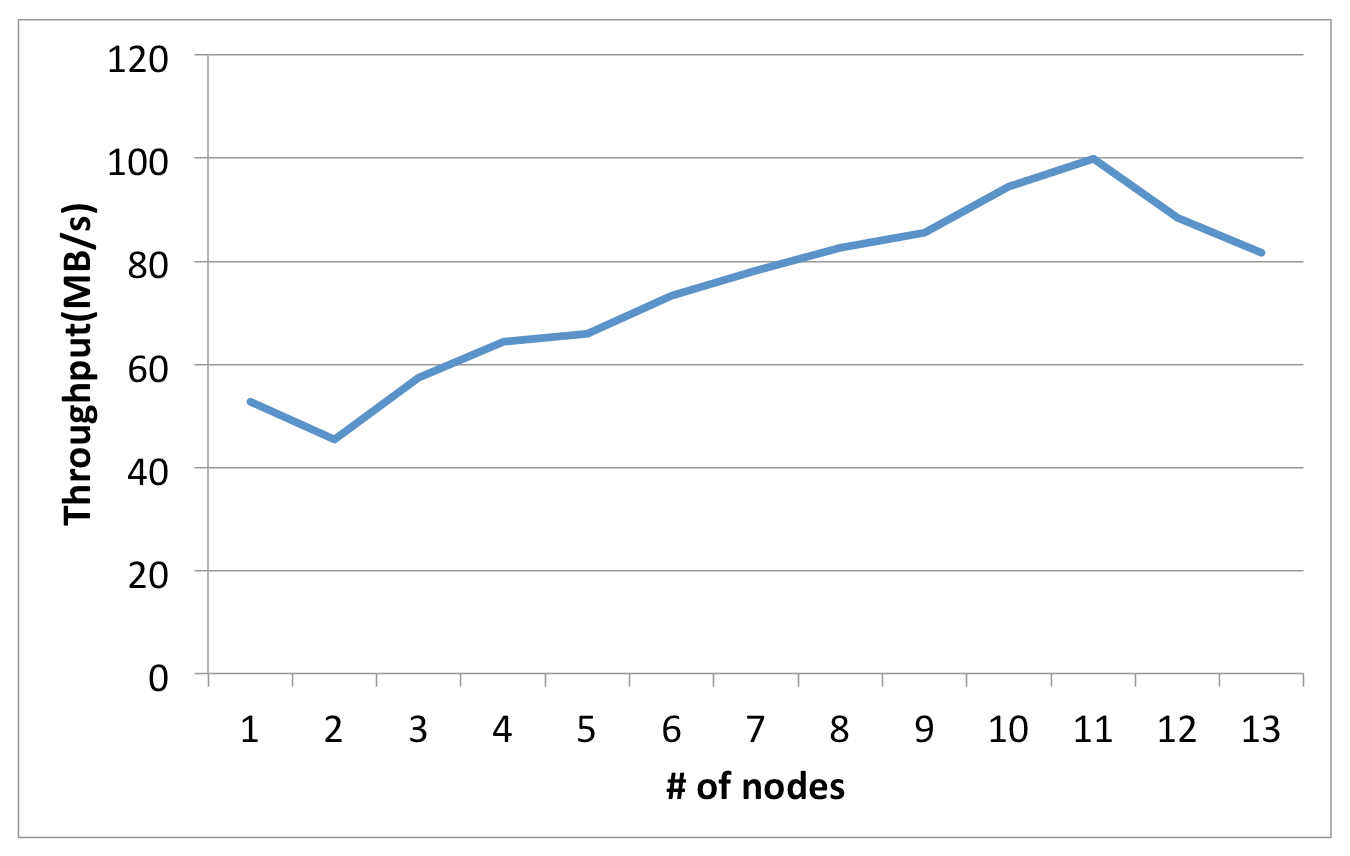
\includegraphics[width=6cm]{../img/AMAZON_to_OUR_LAB}
	\caption{I/O Throughput from AMAZON EC2 to file system inside our lab using sshfs}
	\label{throughput AMAZON to OURLAB}
\end{figure}

\begin{figure}[tb]
	\centering
	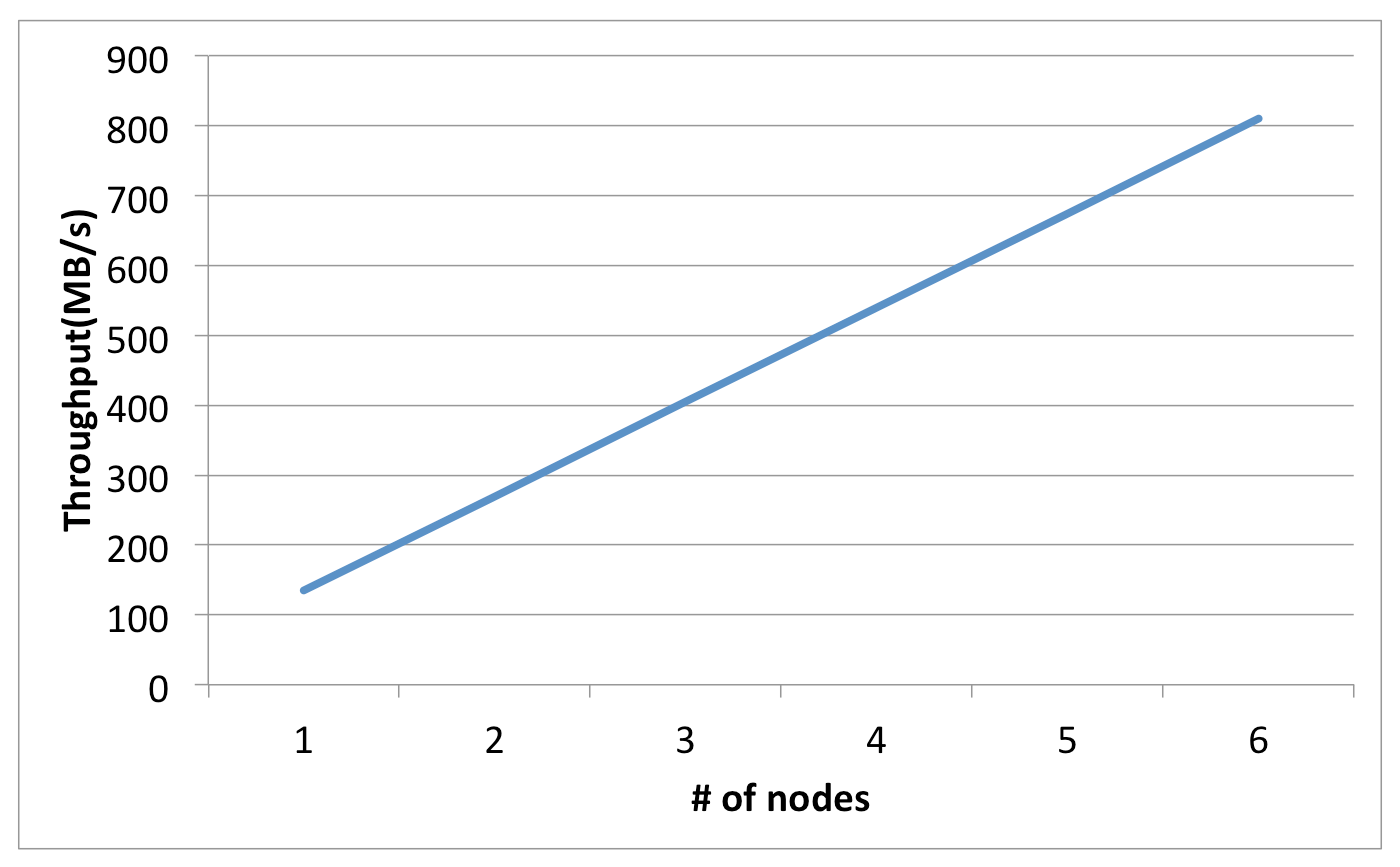
\includegraphics[width=6cm]{../img/point_to_point_AMAZON}
	\caption{point to point connection inside AMAZON}
	\label{point to point connection AMAZON}
\end{figure}

\begin{figure}[tb]
	\centering
	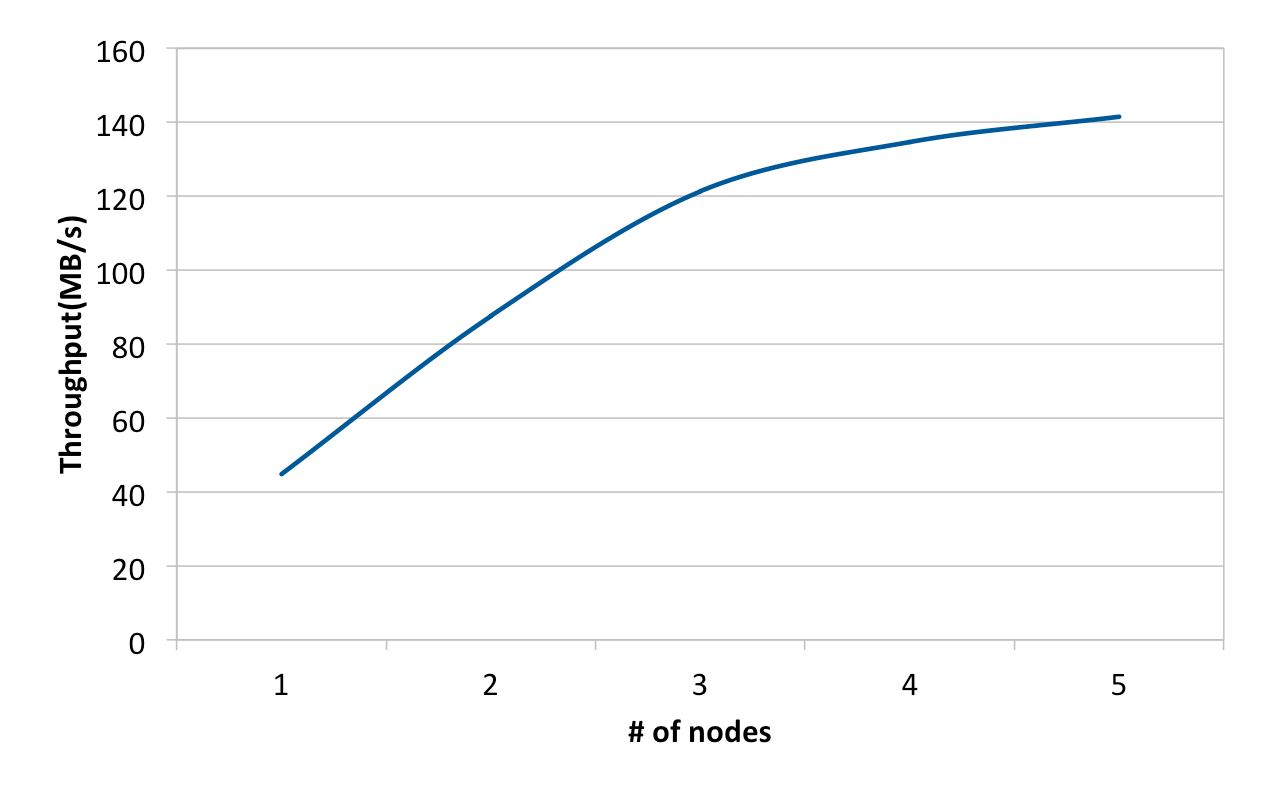
\includegraphics[width=6cm]{../img/point_to_point_lab}
	\caption{point to point connection throughput between AMAZON and our lab}
	\label{point to point connection LAB}
\end{figure}

As we know, throughput gap between interconnection network and Internet is extremely large, also numbers of I/O nodes will affect I/O performance.
We use Iperf\cite{iperf}, which was developed by NLANR/DAST as a modern alternative for measuring TCP and UDP bandwidth performance, and IOR\cite{IOR}, which is widely used for benchmarking parallel file systems using POSIX, MPIIO, or HDF5 interfaces.

Fig.~\ref{throughput TSUBAME} shows I/O throughput between TSUBAME V queue nodes, which run on VM on several shared machines and TSBUAME Lustre file system, which is mounted by using lustre client, it is a interconnection throughput inside TSUBAME supercomputer, we can see that I/O throughput growing as numbers of nodes growing, and the aggregate read and write throughput reach 6-8GB/s with 64 nodes, the same result also can be seen in \cite{checkpointing}.
On the other hand, Fig.~\ref{throughput AMAZON to OURLAB} shows I/O throughput between AMAZON EC2 m3.medium nodes, which have moderate network performance, and a file system machine inside our lab, which has about 1GBit/s Internet access.
Since TSUBAME Lustre can not be accessed outside of TSUBAME because of security problem, instead of TSUBAME Lustre file system, we used a file server inside our lab, which has 1GBit/s internet bandwidth, also because of security problem, we used sshfs\cite{sshfs},which is a filesystem client based on SSH File Transfer Protocol, to mount this file system from AMAZON.
We can see that the I/O throughput also grows as number of nodes grows but the aggregate throughput is only 100-140 MB/s, about 40-80 times smaller than throughput inside TSUBAME.
%From Fig.~\ref{throughput TSUBAME} and Fig.~\ref{throughput AMAZON to TSUBAME Lustre} we can see that the I/O throughput of interconnection inside supercomputer is quit larger than that from AMAZON.
%Also, if we compare the one nodes I/O throughput, 
Also if we compare Fig.~\ref{point to point connection LAB} with Fig.~\ref{throughput AMAZON to OURLAB}, the maximum throughput 
If we move some jobs to AMAZON EC2 with input data stored in TSUBAME Lustre, the execution time will increase because of I/O low throughput,for a data sensitive application, it will be devastating, also according to AMAZON's pay-as-you-go policy\cite{AMAZON_AWS}, longer execution time means more cost.

%But when we compare Fig.~\ref{point to point connection TSUBAME} with FIg.~\ref{point to point connection AMAZON}, the interconnection throughput 
However, if we consider interconnection throughput, as shown in Fig.\ref{point to point connection AMAZON}, although each node can achieve only 1GB/s, the influence between nodes is extremely small, figure shows a perfect linear line also a strong scalability.
Since we can achieve a high interconnection throughput inside a system (HPC system, public cloud), we consider use some nodes as a buffer nodes, using a buffer queue to buffer I/O data and achieve a high throughput.

Although there are some studies about workflow optimization and  balance\cite{Workload}, Since data transfer rate is extremely low in Internet compared with interconnection network and data size processed is extremely large, user do not want to settle their nodes across two systems, so in this model, we just consider the situation that all nodes used for the same job are allocated in the same system.
